%----------------------------------------------------------------------------------------
%	PACKAGES AND OTHER DOCUMENT CONFIGURATIONS
%----------------------------------------------------------------------------------------

\documentclass{article}

\usepackage{fancyhdr} % Required for custom headers
\usepackage{lastpage} % Required to determine the last page for the footer
\usepackage{extramarks} % Required for headers and footers
\usepackage[usenames,dvipsnames]{color} % Required for custom colors
\usepackage{graphicx} % Required to insert images
\usepackage{listings} % Required for insertion of code
\usepackage{courier} % Required for the courier font
\usepackage{lipsum} % Used for inserting dummy 'Lorem ipsum' text into the template
\usepackage{parskip}
% Margins
\topmargin=-0.45in
\evensidemargin=0in
\oddsidemargin=0in
\textwidth=6.5in
\textheight=9.0in
\headsep=0.25in

\linespread{1.1} % Line spacing

% Set up the header and footer
\pagestyle{fancy}
\chead{} % Top left header
\lhead{\hmwkClass\  \hmwkTitle} % Top center head
\rhead{} % Top right header
\lfoot{\lastxmark} % Bottom left footer
\cfoot{} % Bottom center footer
\rfoot{Page\ \thepage\ of\ \protect\pageref{LastPage}} % Bottom right footer
\renewcommand\headrulewidth{0.4pt} % Size of the header rule
\renewcommand\footrulewidth{0.4pt} % Size of the footer rule

\setlength\parindent{0pt} % Removes all indentation from paragraphs

%----------------------------------------------------------------------------------------
%	CODE INCLUSION CONFIGURATION
%----------------------------------------------------------------------------------------

% \definecolor{MyDarkGreen}{rgb}{0.0,0.4,0.0} % This is the color used for comments
\lstloadlanguages{C} % Load C syntax for listings, for a list of other languages supported see: ftp://ftp.tex.ac.uk/tex-archive/macros/latex/contrib/listings/listings.pdf
\lstset{language=C,frame=single,keywordstyle=[1]\color{Blue}\bf} % Use C in this example      



\newcommand{\csnippet}[2]{
\begin{itemize}
\item[]\lstinputlisting[caption=#2,label=#1]{#1.c}
\end{itemize}
}

%----------------------------------------------------------------------------------------
%	DOCUMENT STRUCTURE COMMANDS
%----------------------------------------------------------------------------------------

% Header and footer for when a page split occurs within a problem environment
\newcommand{\enterProblemHeader}[1]{
\nobreak\extramarks{#1}{#1 continued on next page\ldots}\nobreak
\nobreak\extramarks{#1 (continued)}{#1 continued on next page\ldots}\nobreak
}

% Header and footer for when a page split occurs between problem environments
\newcommand{\exitProblemHeader}[1]{
\nobreak\extramarks{#1 (continued)}{#1 continued on next page\ldots}\nobreak
\nobreak\extramarks{#1}{}\nobreak
}

\setcounter{secnumdepth}{0} % Removes default section numbers
\newcounter{homeworkProblemCounter} % Creates a counter to keep track of the number of problems

\newcommand{\homeworkProblemName}{}
\newenvironment{homeworkProblem}[1][Problem \arabic{homeworkProblemCounter}]{ % Makes a new environment called homeworkProblem which takes 1 argument (custom name) but the default is "Problem #"
\stepcounter{homeworkProblemCounter} % Increase counter for number of problems
\renewcommand{\homeworkProblemName}{#1} % Assign \homeworkProblemName the name of the problem
\section{\homeworkProblemName} % Make a section in the document with the custom problem count
\enterProblemHeader{\homeworkProblemName} % Header and footer within the environment
}{
\exitProblemHeader{\homeworkProblemName} % Header and footer after the environment
}

\newcommand{\problemAnswer}[1]{ % Defines the problem answer command with the content as the only argument
\noindent\framebox[\columnwidth][c]{\begin{minipage}{0.98\columnwidth}#1\end{minipage}} % Makes the box around the problem answer and puts the content inside
}

\newcommand{\homeworkSectionName}{}
\newenvironment{homeworkSection}[1]{ % New environment for sections within homework problems, takes 1 argument - the name of the section
\renewcommand{\homeworkSectionName}{#1} % Assign \homeworkSectionName to the name of the section from the environment argument
\subsection{\homeworkSectionName} % Make a subsection with the custom name of the subsection
\enterProblemHeader{\homeworkProblemName\ [\homeworkSectionName]} % Header and footer within the environment
}{
\enterProblemHeader{\homeworkProblemName} % Header and footer after the environment
}

%----------------------------------------------------------------------------------------
%	NAME AND CLASS SECTION
%----------------------------------------------------------------------------------------

\newcommand{\hmwkTitle}{Assignment\ \#4} % assignment title
\newcommand{\hmwkDueDate}{Monday,\ December\ 8,\ 2014} % due date
\newcommand{\hmwkClass}{Programming Concurrent Systems} % class
\newcommand{\hmwkClassTime}{} % lecture time
\newcommand{\hmwkClassInstructor}{} % lecturer
\newcommand{\hmwkAuthorName}{Alyssa - Ilias} %name

%----------------------------------------------------------------------------------------
%	TITLE PAGE
%----------------------------------------------------------------------------------------

\title{
\vspace{2in}
\textmd{\textbf{\hmwkClass:\ \hmwkTitle}}\\
\normalsize\vspace{0.1in}\small{Due\ on\ \hmwkDueDate}\\
\vspace{0.1in}\large{\textit{\hmwkClassInstructor\ \hmwkClassTime}}
\vspace{3in}
}

\author{\textbf{\hmwkAuthorName}}


%----------------------------------------------------------------------------------------

\begin{document}

\maketitle

%----------------------------------------------------------------------------------------
%	TABLE OF CONTENTS
%----------------------------------------------------------------------------------------

%\setcounter{tocdepth}{1} % Uncomment this line if you don't want subsections listed in the ToC

%\newpage
%\tableofcontents
\newpage

%----------------------------------------------------------------------------------------
%	Introduction
%----------------------------------------------------------------------------------------
\begin{homeworkProblem}[Introduction]

This assignment asked us to perform experiments using OpenACC. In this report, we present results from
the first two parts: first, experiments from accelerating our heat dissipation code, and then some
results from the provided matmul code.

\end{homeworkProblem}
%----------------------------------------------------------------------------------------
%	Heat
%----------------------------------------------------------------------------------------

% To have just one problem per page, simply put a \clearpage after each problem

\begin{homeworkProblem}[Heat dissipation | OpenACC]
\textbf{Solution description}

Our solution this time is based on the reference code, due to issues with the extensive
use of pointer arithmetic in our original code. We used the adapted version of the reference
code from Franz Geiger, which fixes compilation issues with the PGI compiler due to the lack
of support for C99 multidimensional variable-length arrays.

We rearranged the code to remove unnecessary smearing iterations from the computation loops,
and to move it all into a single function for simplicity.

We copy all three matrices (the conduction data, and the source/destination matrices) in at
the start of the main loop. The destination data is largely garbage at this point, and so a
small performance improvement could be obtained by only copying in the (smeared) edges, but
for simplicity we didn't do thisa.

\csnippet{main}{Main loop}

We parallelized the main dissipation computation, including the smearing. Note that we use
the \texttt{present} directive, which avoids an unnecessary copy but also makes the GPU
aware of the swapped destination/source pointers.

\csnippet{compute}{Dissipation computation}

And we also parallelized the reduction step, using OpenACC's directive:

\csnippet{reduction}{Reduction using acc directive}

The use of the \texttt{independent} directive on the pragmas informs PGI that the loops do not
have data dependencies on each other.

(We also included OpenMP directives, but the resulting code is slower than our original OpenMP
code, so we didn't use it.)

\textbf{Evaluation - Experiments}

We run our experiments on the DAS-4 system. For pthreads/OpenMP, we used a normal node which has 8 physical cores.
For the OpenACC results, we used the nvidia (CUDA) backend of the PGI compiler, and ran the result on the DAS-4
systems with either a GTX480 or a Tesla C2050. The limited availability of the nodes with other GPU types made it
difficult to experiment with them.

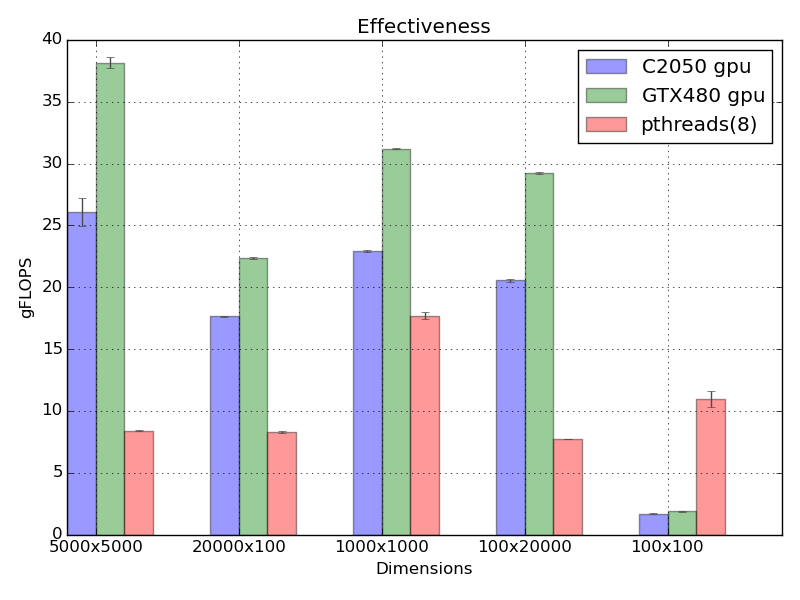
\includegraphics[width=0.75\columnwidth]{effectivness.png}

The figure above shows the effectiveness of the parallelisation. The experiments were made with the following parameters:

\begin{verbatim}
./heat -e 0.0 -i 2000 -k 2001
\end{verbatim}

Notice how, for the first time, effectiveness did not necessarily equate to small execution time, due to the communication overhead.

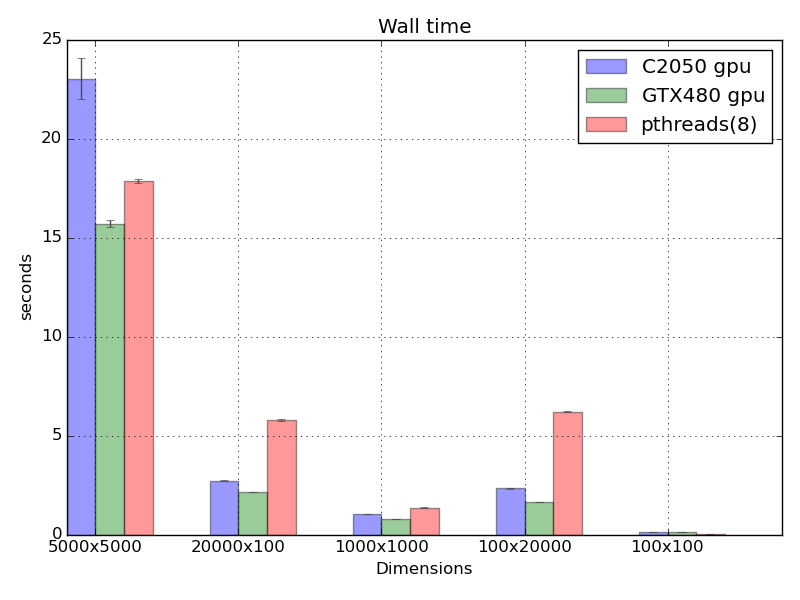
\includegraphics[width=0.75\columnwidth]{walltime.png} 

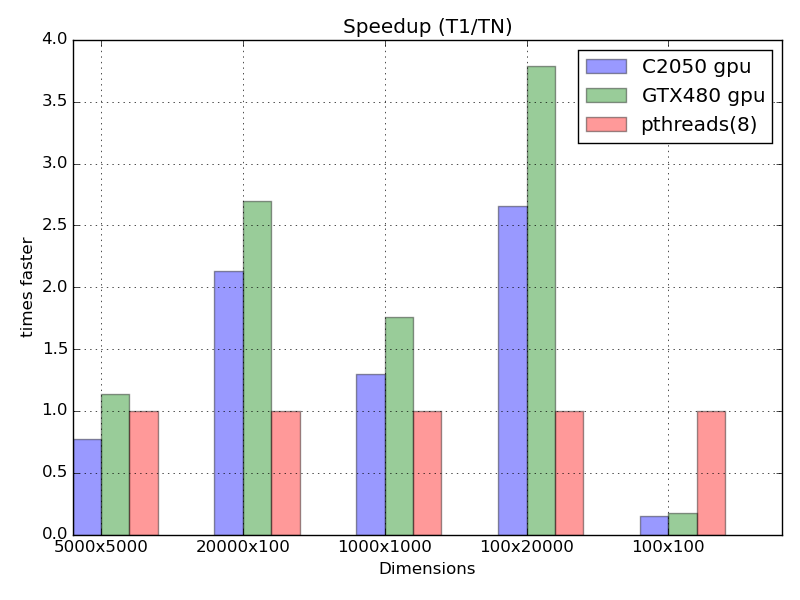
\includegraphics[width=0.75\columnwidth]{speedup_heat.png} 

A good GPU implementation of this problem would proceed using tiles/blocks (since the neighbours which are needed
by each computation are in all directions), ideally copying each block into shared memory rather than accessing global
memory repeatedly. Unfortunately, PGI doesn't support the OpenACC 2.0 \texttt{tile} pragma, and in any case, the
details of shared memory are not exposed.

We did, however, perform some experiments to try working out the optimal combination of gang, worker and vector
sizes to use. Unfortunately, these results were invalidated shortly before submitting this report when we realised
that we'd made a fundamental mistake in the loop iterations (we were iterating over the horizontal direction in the
outer loop, rather than the vertical one), but we present an example graph showing an example portion of our results
from these experiments anyway (PGI assigns the workers/vectors to dimensions of \texttt{threadIdx}, so the symmetric
nature of the graph is to be expected):

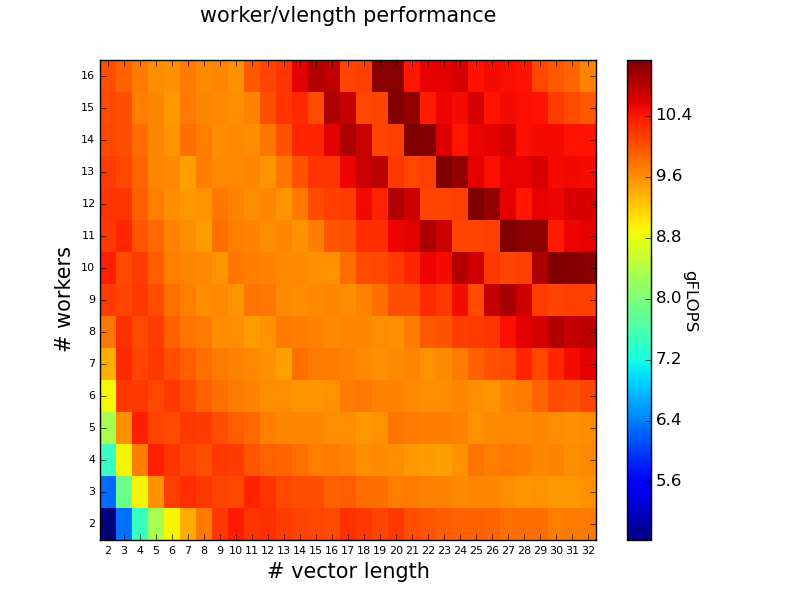
\includegraphics[width=0.75\columnwidth]{heat.png}

The same mistake is present in the 3 charts below, showing the effectiveness, walltime and speedup of the code
with reductions at every step (\texttt{-k 1}):

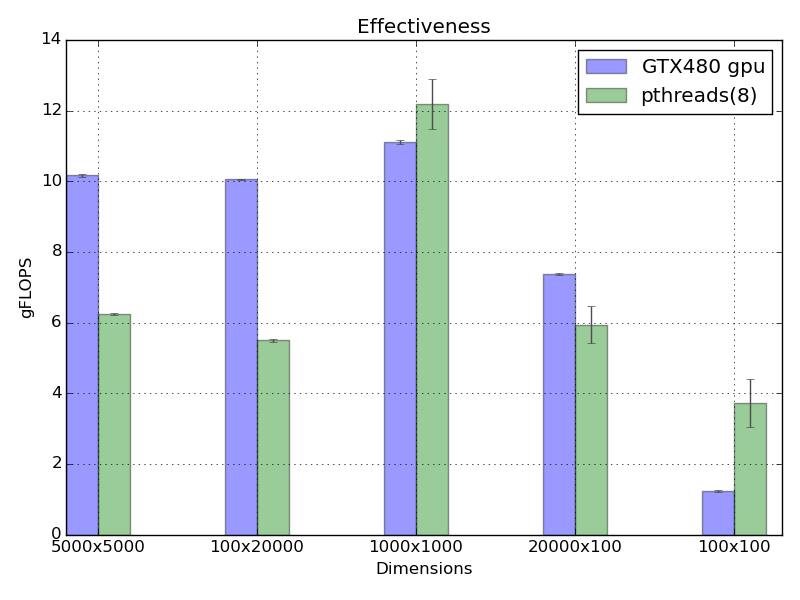
\includegraphics[width=0.75\columnwidth]{effectivness_withreductions.png} 

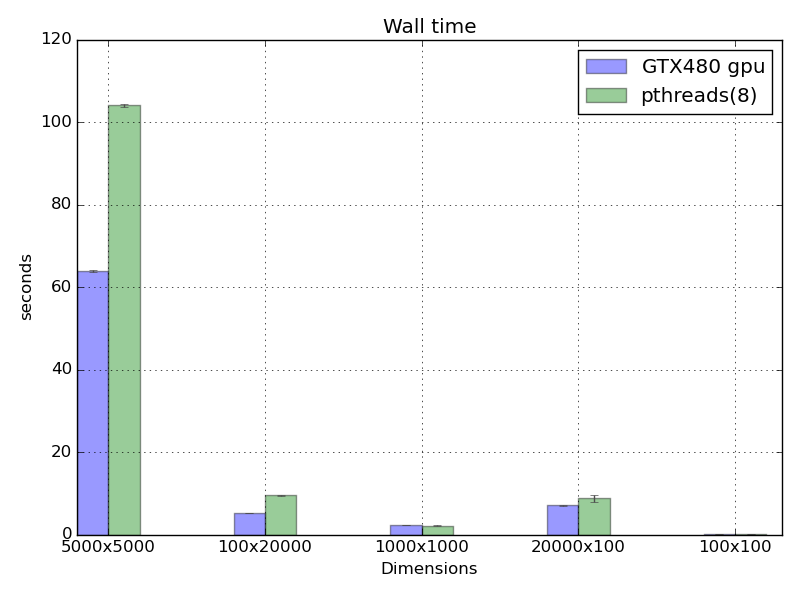
\includegraphics[width=0.75\columnwidth]{walltime_withreductions.png}

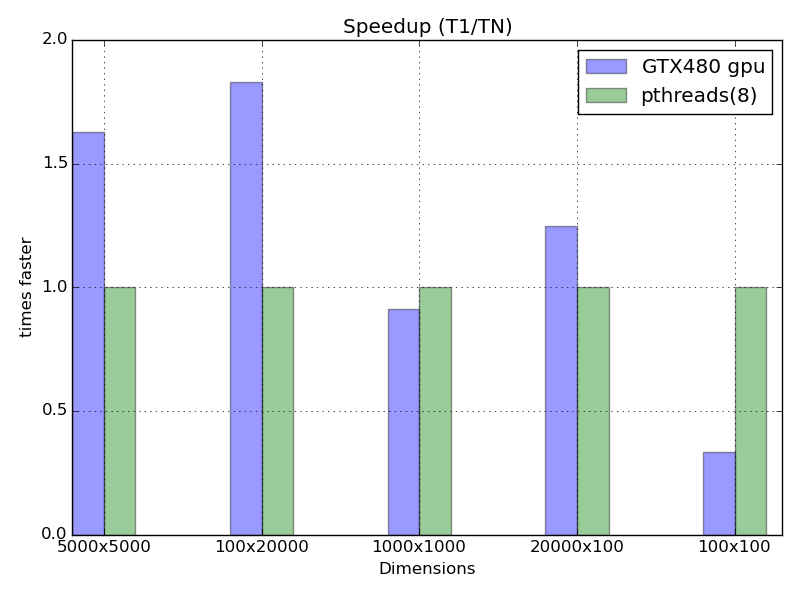
\includegraphics[width=0.75\columnwidth]{speedup_withreductions.png} 

\textbf{Discussion}

We can use \texttt{pgaccelinfo} to investigate attributes such as the warp size, maximum block size,
available shared memory, etc, which we didn't yet find particularly useful during this assignment due to
the limitations of OpenACC. Some example output, from a node with a GTX480:

\begin{verbatim}
Total Constant Memory:         65536
Total Shared Memory per Block: 49152
Registers per Block:           32768
Warp Size:                     32
Maximum Threads per Block:     1024
Maximum Block Dimensions:      1024, 1024, 64
Maximum Grid Dimensions:       65535 x 65535 x 65535
\end{verbatim}

To make sure our compute code is compiled optimally, we consider the \texttt{-Minfo} output, which gives
us information about where Tesla code is generated (and when loops are not vectorized). For example,
for the reduction loop (the outer loop is on line 124, and the inner loop on line 127):

\begin{verbatim}
    124, Generating present(dst[:?])
         Generating present(src[:?])
         Accelerator kernel generated
        125, #pragma acc loop gang /* blockIdx.x */
        127, #pragma acc loop vector(256) /* threadIdx.x */
        132, Min reduction generated for tmin
        135, Max reduction generated for tmax
        138, Sum reduction generated for tavg
        141, Max reduction generated for maxdiff
    124, Generating Tesla code
    127, Loop is parallelizable
\end{verbatim}

We used the \texttt{PGI\_ACC\_TIME} environment variable to confirm that our code was running correctly (for example,
that it was only reaching the \texttt{enter data} region once). The output agrees with this, and justifies our earlier
decision not to consider copying in portions of matrices (or using \texttt{create} and doing the work on the GPU)
due to the massive differences in time between the first data region (copying data in) and the first compute region.
It also shows that the computation times for the blocks are largely balanced, with only small differences between them.
One example (for a $5000\times5000$ matrix, and the above parameters) is provided below:

\begin{verbatim}
71: data region reached 1 time
    71: data copyin transfers: 36
         device time(us): total=421 max=17 min=3 avg=11
86: data region reached 2000 times
86: compute region reached 2000 times
    86: kernel launched 2000 times
        grid: [5000]  block: [128]
         device time(us): total=15,220,640 max=7,638 min=7,600 avg=7,610
\end{verbatim}

We can get some insight into how the problem is being split up by PGI by considering the grid/block sizes above, but
also more interestingly, for the reduction, which is done very simplistically, using a reduction kernel launched after
a main kernel. Again, from the same example:

\begin{verbatim}
124: kernel launched 1 time
    grid: [5000]  block: [256]
     device time(us): total=3,105 max=3,105 min=3,105 avg=3,105
124: reduction kernel launched 1 time
    grid: [4]  block: [256]
     device time(us): total=25 max=25 min=25 avg=25
\end{verbatim}

\texttt{PGI\_ACC\_DEBUG} gives somewhat similar (but more detailed) information, although without the timings.

\end{homeworkProblem}

%----------------------------------------------------------------------------------------
%	Merge
%----------------------------------------------------------------------------------------

\begin{homeworkProblem}[Matmul]

We discussed a lot of the suggestions in the matmul portion of the assignment (e.g., \texttt{PGI\_ACC\_TIME}) above,
so we won't discuss these details again for the less interesting matmul case, but rather simply present our results.

You can observe that, if we only perform one iteration, then the time taken for the multiplication scales reasonably
well for the number of elements with both OpenACC and OpenMP, but OpenMP is considerably faster:

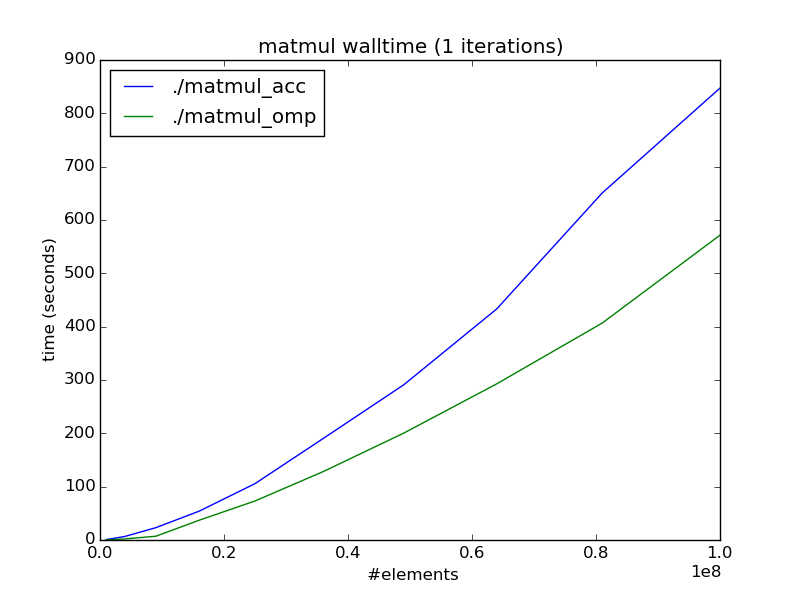
\includegraphics[width=0.75\columnwidth]{bigfig.png} 

And this is similar for a far larger number of elements:

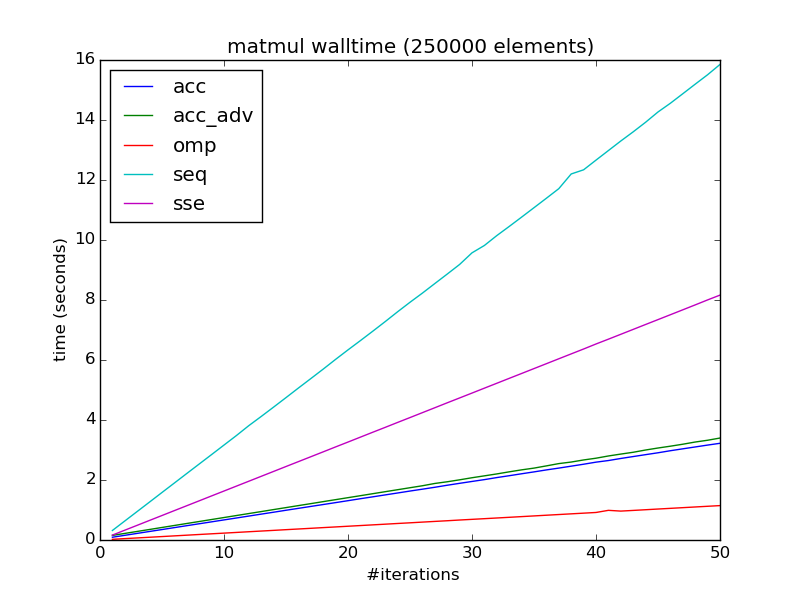
\includegraphics[width=0.75\columnwidth]{fig.png}

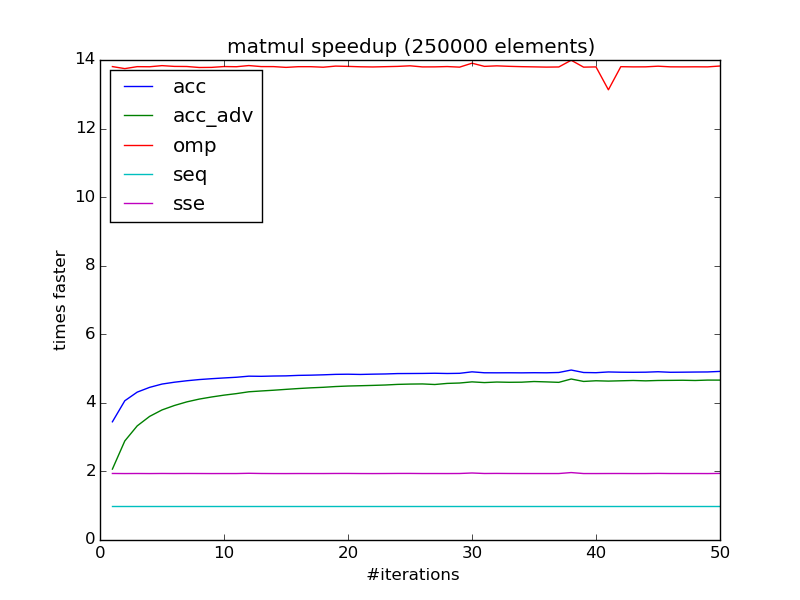
\includegraphics[width=0.75\columnwidth]{speedup.png} 

And even with a huge number of elements, the situation is similar. OpenACC is (reassuringly) clearly much better than at least the sequential versions:

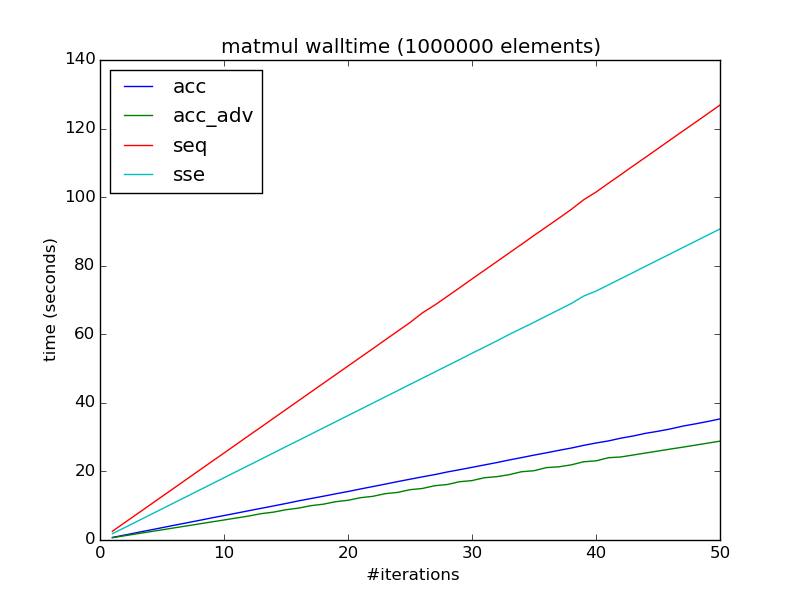
\includegraphics[width=0.75\columnwidth]{matmul_more_elements.png}

\end{homeworkProblem}

%----------------------------------------------------------------------------------------

\end{document}
